\documentclass[portrait, a1paper, fontscale=0.5]{baposter}

\usepackage[utf8]{inputenc}
\usepackage{graphicx}

\definecolor{bgcolorone}{RGB}{225,225,225}
\definecolor{bgcolortwo}{RGB}{225,225,225}
\definecolor{bordercolor}{RGB}{153,153,153}
\definecolor{headercolorone}{RGB}{255,255,255}
\definecolor{headercolortwo}{RGB}{255,255,255}
\definecolor{headerfontcolor}{RGB}{7,67,145}
\definecolor{boxcolorone}{RGB}{200,200,200}

\pdfinfo
{
	/Title (SNA)
	/Author (P. Kus, P. Karban, F. Mach)
}

\begin{document}

\background{}

\begin{poster}{
	grid=false,
	columns=3,
	background=plain,
	bgColorOne=bgcolorone,
	%bgColorTwo=bgcolortwo,
	borderColor=bordercolor,
	headerColorOne=headercolorone,
	headerColorTwo=headercolortwo,
	headerFontColor=headerfontcolor,
	boxColorOne=boxcolorone,
	headershape=roundedright,
	headerfont=\large\sc,
	textborder=roundedleft,
	background=user,
	headerborder=open,
	boxshade=none
}
{
\includegraphics[width=17em]{fel.pdf}}
{\huge\textsc{\textcolor{headerfontcolor}{Solving nonlinear coupled problems using Agros2D}}\vspace{0.75em}}
{\Large{\textcolor{headerfontcolor}{P. Kus$^{1}$, P. Karban$^{2}$ and F. Mach$^{1, 2}$\\{\large $^{1}$ \textit{Institute of Thermomechanics, Academy of Sciences CR, v. v. i.}}\\{\large $^{2}$ \textit{Faculty of Electrical Engineering, University of West Bohemia}}}}}
{
\includegraphics[width=7em]{it.png}}

\headerbox{About Agros2D}{name=about,column=0,row=0}{
Agros2D is a multiplatform C++ application for the solution of partial differential equations (PDE) based on the Hermes library, developed by the hpfem.org group at the University of West Bohemia in Pilsen. Hermes library is developed at University od Reno in Nevada. Agros2D is distributed under the GNU General Public License.
}

\headerbox{Supported physical fields}{name=fields,column=0,row=0,below=about}{
\begin{itemize} \itemsep1pt \parskip0pt \parsep0pt
\item Electrostatic fields
\item Electric current fields
\item Magnetic fields (steady state, harmonic and transient analysis)
\item High frequency electromagnetic fields - in development
\item Temperature fields (steady state and transient analysis)
\item Acoustic field (harmonic and transient analysis)
\item Linear thermo-elasticity
\item Incompressible flow (steady state and transient analysis) - in development
\end{itemize}
}

\headerbox{Key Features}{name=features,column=0,row=0,below=fields}{
\begin{itemize} \itemsep1pt \parskip0pt \parsep0pt
\item Steady state, transient and harmonic analysis
\item Curvilinear elements
\item Arbitrary level hanging nodes
\item Multimesh assembling
\item Automatic hp-adaptivity
\end{itemize}
}

\headerbox{Simple GUI control}{name=gui,column=0,row=0,below=features}{
\begin{itemize} \itemsep1pt \parskip0pt \parsep0pt
\item Interactive geometry definition
\item AutoCAD DXF (Drawing Exchange Format) import and export
\item Visualization of field variables
\item Extraction of local values
\item Calculation of surface and volume integrals
\item Export of charts, data, and images
\item Export movies (transient analysis)
\item Scripting support (based on Python language)
\item Remote control
\end{itemize}
}

\headerbox{Optimization}{name=optimization,column=1,row=0,span=2}{
\begin{center}
	\begin{minipage}{5em}
		\centering
		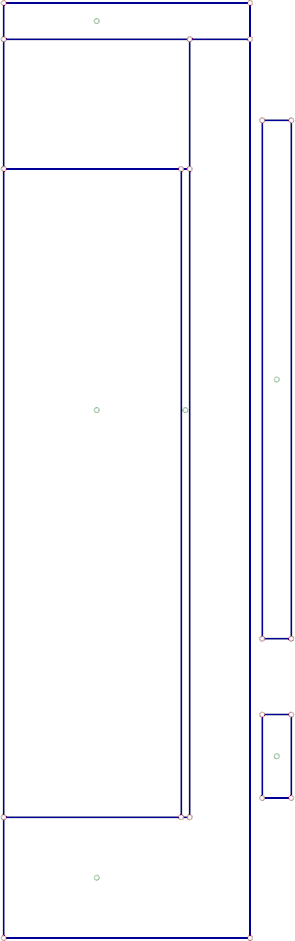
\includegraphics[width=4em]{optimization/variant_1.png}
	\end{minipage}
	\begin{minipage}{5em}
		\centering
		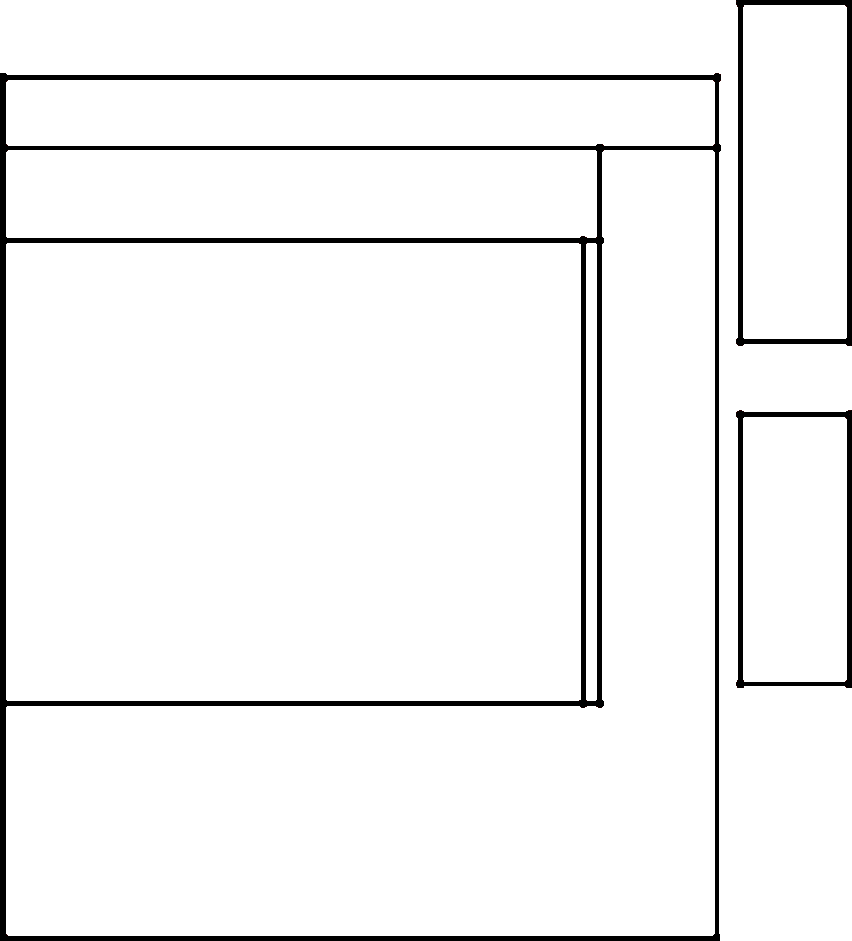
\includegraphics[width=4em]{optimization/variant_2.png}
	\end{minipage}
	\begin{minipage}{5em}
		\centering
		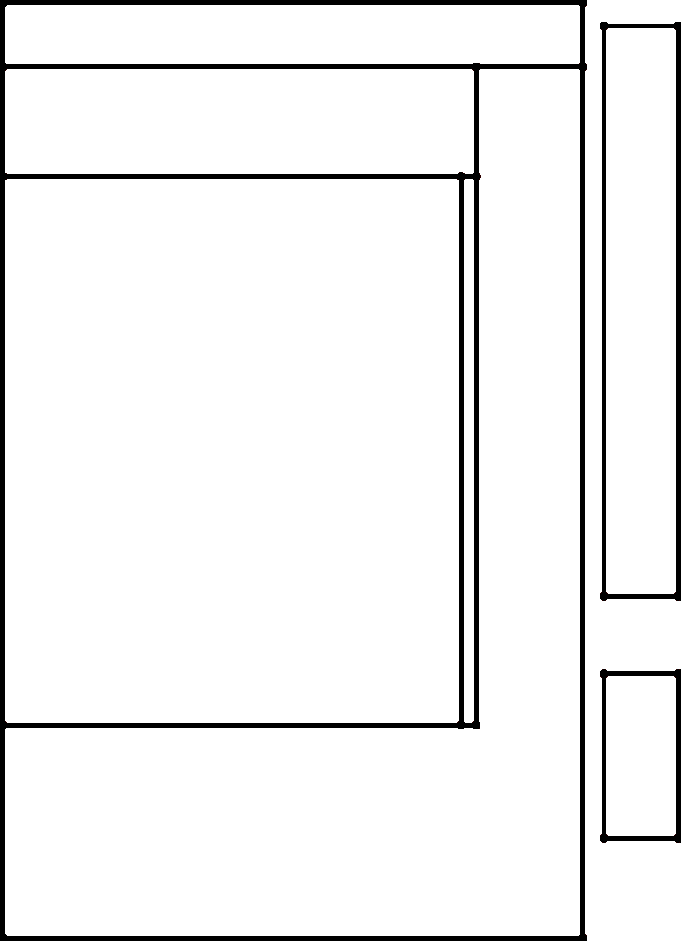
\includegraphics[width=4em]{optimization/variant_3.png}
	\end{minipage}
	\begin{minipage}{5em}
		\centering
		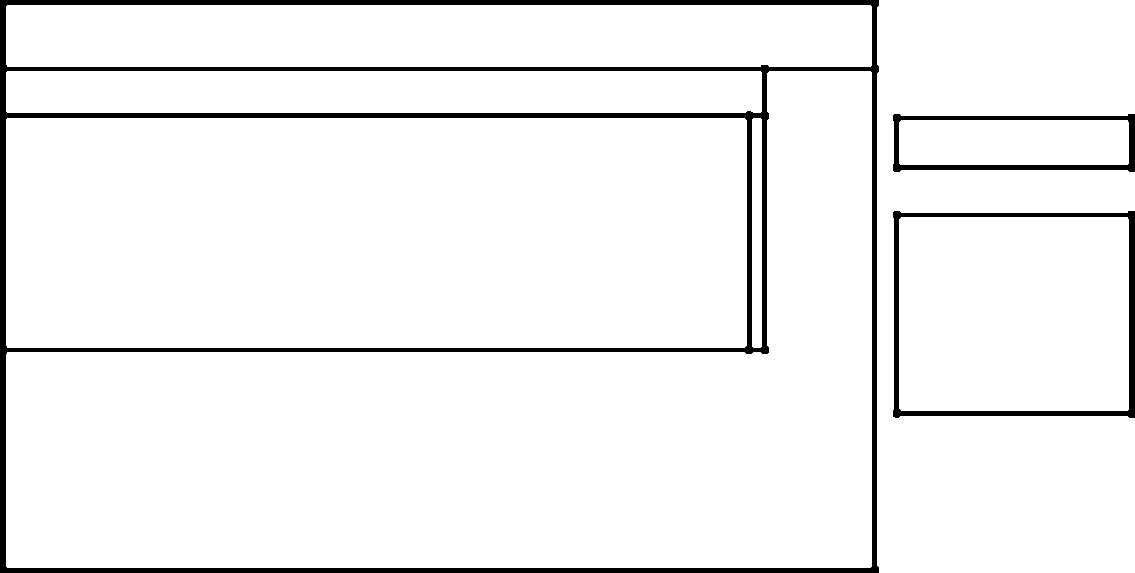
\includegraphics[width=4em]{optimization/variant_4.png}
	\end{minipage}
	\begin{minipage}{5em}
		\centering
		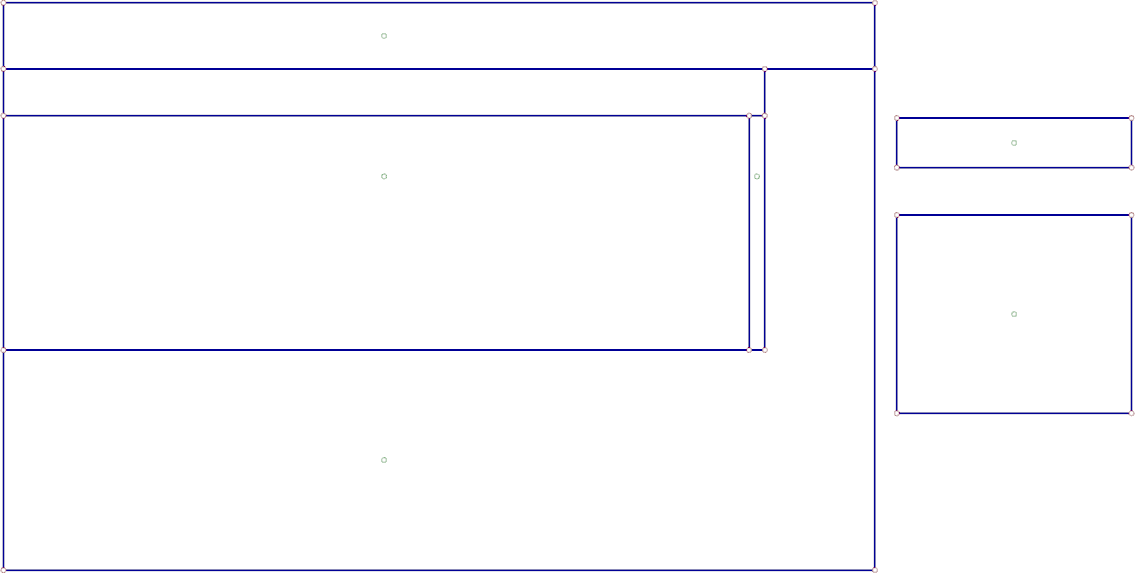
\includegraphics[width=4em]{optimization/variant_5.png}
	\end{minipage}
	\begin{minipage}{5em}
		\centering
		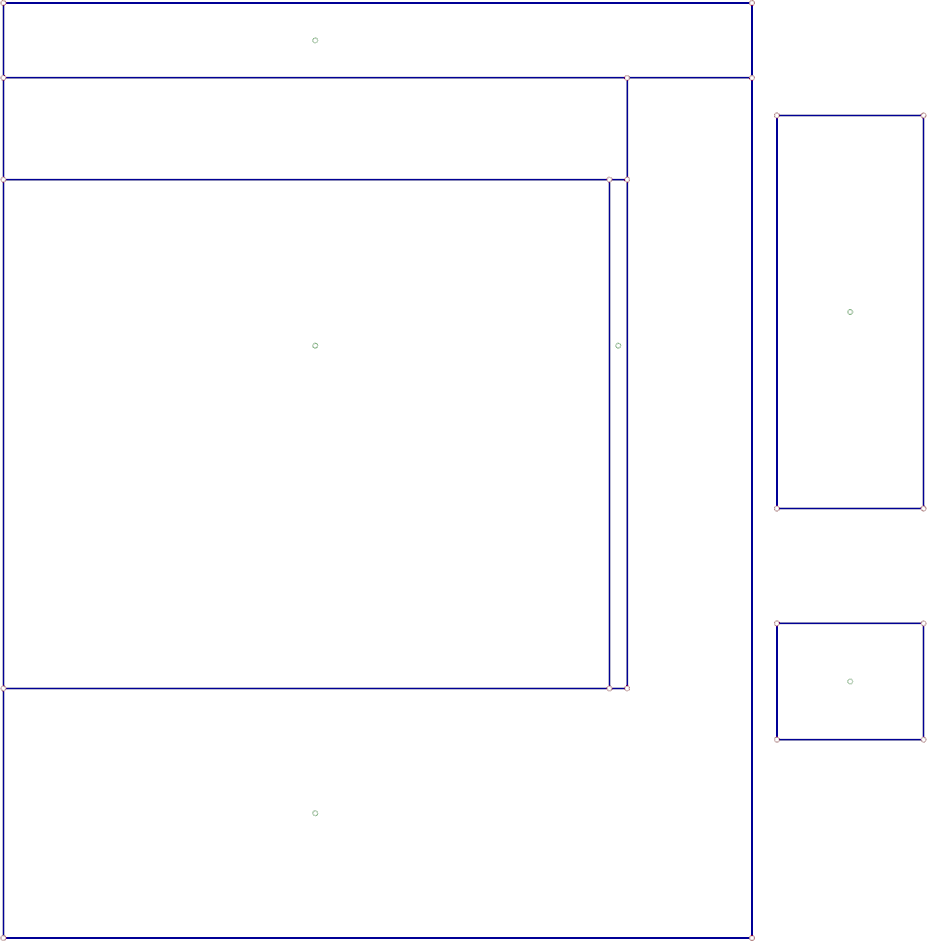
\includegraphics[width=4em]{optimization/variant_6.png}
	\end{minipage}
	\begin{minipage}{5em}
		\centering
		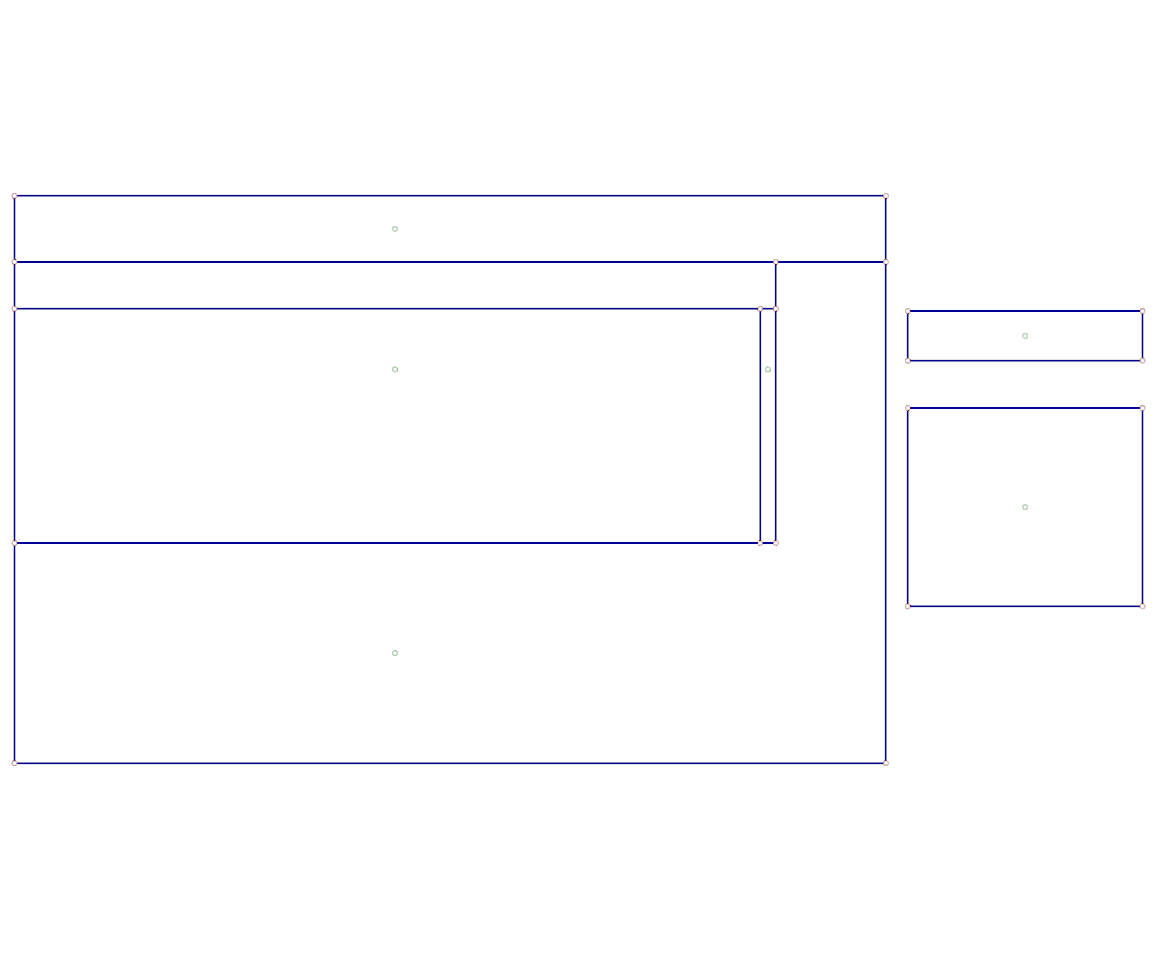
\includegraphics[width=4em]{optimization/variant_7.png}
	\end{minipage}
\end{center}

\begin{center}
	\begin{minipage}{10em}
		\centering
		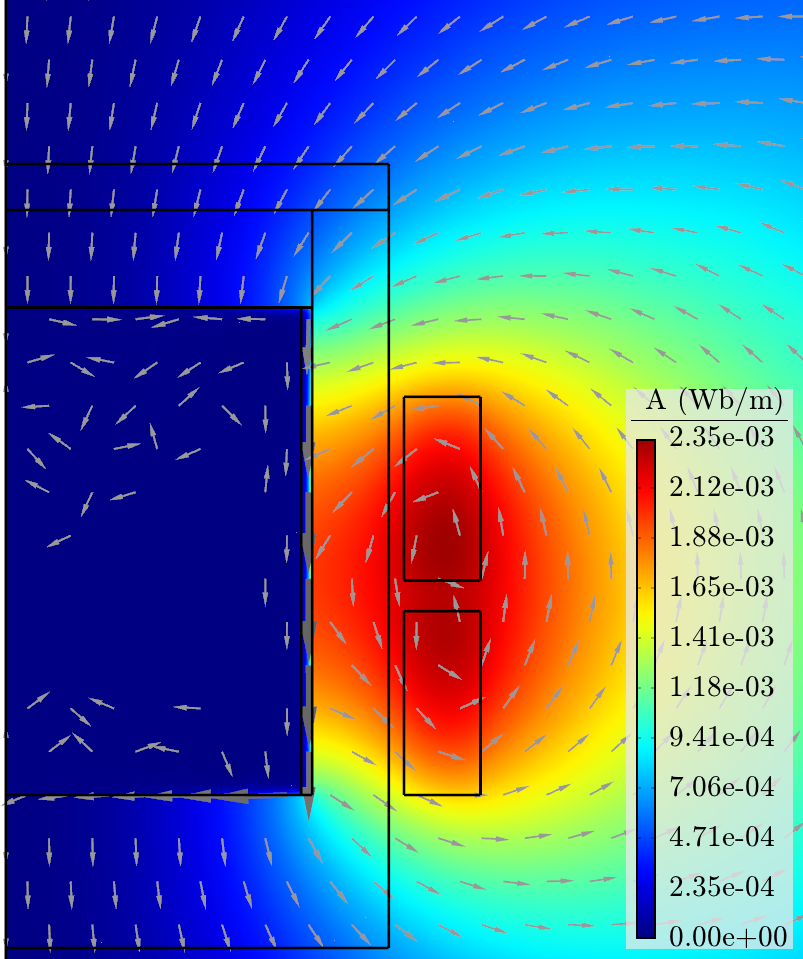
\includegraphics[height=13em]{optimization/magnetic_field.png}
	\end{minipage}
	\begin{minipage}{10em}
		\centering
		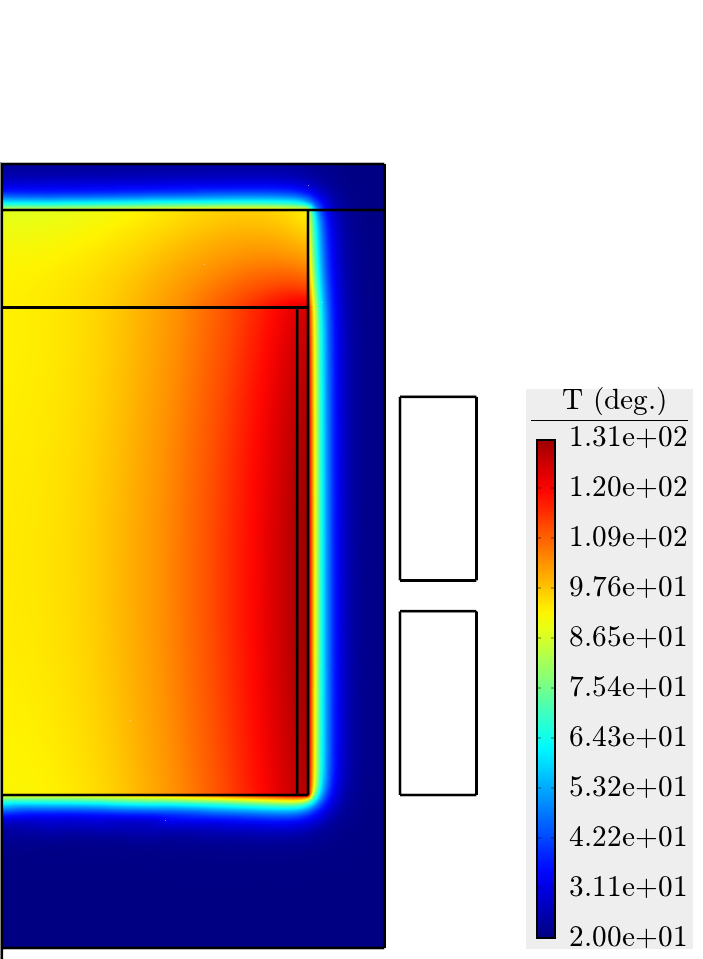
\includegraphics[height=13em]{optimization/temperature_field.png}
	\end{minipage}
	\begin{minipage}{30em}
		Lorem ipsum dolor sit amet, consectetur adipiscing elit. Sed sit amet felis nunc, ut ornare orci. Cras enim velit, tincidunt sit amet dignissim at, tincidunt in nunc. Donec facilisis metus nec dui tempus mattis. Vestibulum enim mi, consectetur gravida sagittis vel, facilisis a orci. Quisque eget dolor risus. In id purus dictum nisi viverra imperdiet sed vel nulla. Ut accumsan, orci in auctor ultricies, dolor massa congue lorem, nec gravida ante nisl sed lacus. Etiam in ipsum in nisl euismod posuere at vitae ligula. Aliquam erat volutpat. Aenean et ante erat, vel vulputate risus. Aenean facilisis tempor auctor. Integer ullamcorper felis at mi fermentum cursus. Maecenas ut diam non libero fermentum pellentesque. Nullam in arcu enim, quis bibendum ipsum. Quisque scelerisque porttitor nibh, ac tincidunt lacus blandit tincidunt.
	\end{minipage}
\end{center}

\begin{center}
	\begin{minipage}{25em}
		Phasellus mattis enim vitae nisl cursus vel vestibulum urna scelerisque. Integer dolor eros, scelerisque vel sodales sit amet, porta quis purus. Curabitur varius imperdiet arcu eget faucibus. Nunc sollicitudin hendrerit neque, ut interdum lacus bibendum at. Vivamus quam orci, mollis id dapibus at, interdum sed dolor. Aliquam at erat nisl, placerat rutrum mauris. Praesent ipsum tellus, venenatis pharetra lacinia id, elementum quis libero.
	\end{minipage}
	\begin{minipage}{25em}
		\centering
		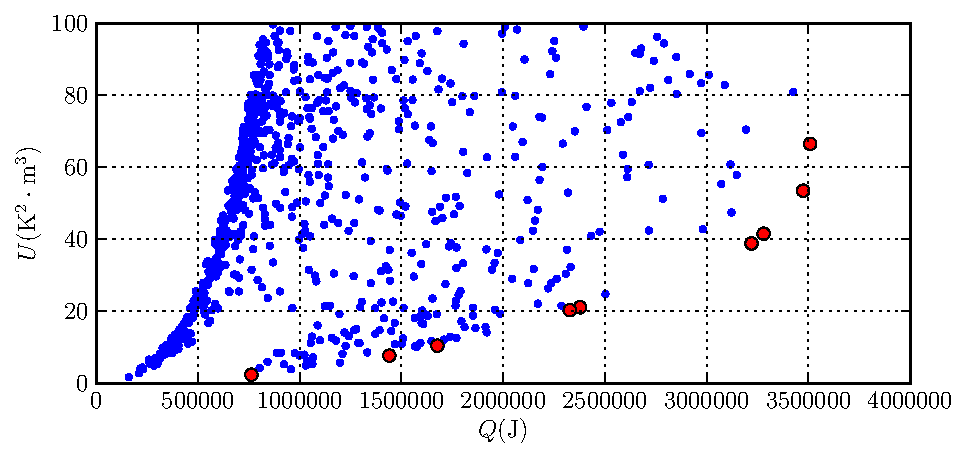
\includegraphics[width=25em]{optimization/results.pdf}
	\end{minipage}
\end{center}
}

\headerbox{Particle tracing}{name=particle_tracing,column=1,row=0,span=2,below=optimization}{
}
\headerbox{References}{name=references,column=1,row=0,span=2,below=particle_tracing}{
}
\end{poster}
\end{document}